\documentclass[11pt,xcolor=svgnames]{beamer}
\usepackage{amsmath}
\usepackage{amssymb}
\usepackage{amsfonts}
\usepackage{dsfont,natbib,setspace,changepage,multirow}
\mode<presentation>

% replaces beamer foot with simple page number
\setbeamertemplate{navigation symbols}{}
\setbeamerfont{frametitle}{series=\bfseries,size=\normalsize}
\setbeamercolor{frametitle}{fg=Black}

\setbeamertemplate{footline}{
  \raisebox{5pt}{\makebox[\paperwidth]{\hfill\makebox[20pt]{\color{gray}\scriptsize\insertframenumber}}}}

\usepackage{algorithm}
\usepackage{algorithmic}

% colors
\newcommand{\theme}{\color{DarkRed}}
\newcommand{\bk}{\color{black}}
\newcommand{\rd}{\color{red}}
\newcommand{\fg}{\color{ForestGreen}}
\newcommand{\bl}{\color{blue}}
\newcommand{\gr}{\color{black!50}}
\newcommand{\sg}{\color{DarkSlateGray}}
\newcommand{\nv}{\color{Navy}}
\setbeamercolor{itemize item}{fg=gray}

% common math markups
\newcommand{\bs}[1]{\boldsymbol{#1}}
\newcommand{\mc}[1]{\mathcal{#1}}
\newcommand{\mr}[1]{\mathrm{#1}}
\newcommand{\bm}[1]{\mathbf{#1}}
\newcommand{\ds}[1]{\mathds{#1}}
\newcommand{\indep}{\perp\!\!\!\perp}
\def\plus{\texttt{+}}
\def\minus{\texttt{-}}
\DeclareMathOperator*{\argmin}{arg\,min}

% spacing and style shorthand
\setstretch{1.1}

\title{Persado Email Subject Lines}
\subtitle{Digital and Algorithmic Marketing (37304-01)}
\author{Brian Chingono, Will Clark, Matthew DeLio, Jonathan Stevens}
% \institute{University of Chicago Booth School of Business}
\institute{
\includegraphics[width=0.5\textwidth]{university_of_chicago_booth_business_school.png}}
\date{\today}

\begin{document}

\begingroup % remove page number from title slide (probably a simpler way to get this done but it works)
\renewcommand{\insertframenumber}{}
 \begin{frame}
  \addtocounter{framenumber}{-1}
  \titlepage
 \end{frame}
\endgroup

% Didn't want on title page because we'd duplicate the phoenix
{\usebackgroundtemplate{
\includegraphics[height=\paperheight]{phoenix}}

\begin{frame}

Modeling objectives:
\begin{itemize}
\item Predict click behavior out of sample\\\textit{\fg select variables via cross validation}
\item Prefer simplicity/parsimony to complexity\\\textit{\fg choose a small model}
\item Main effects matter more than interaction effects\\\textit{\fg impose a bias toward main effects}
\end{itemize}

\end{frame}

\begin{frame}

The model:
\[ \frac{\textsf{Pr}(\text{click}=1)}{1-\textsf{Pr}(\text{click}=1)} = \beta_0 + \underbrace{\sum_{j=1}^{p} x_j \beta_j}_{\text{main effects}} + \underbrace{\sum_{j=1}^p \sum_{k=1}^{j} x_j x_k \beta_{jk}}_{\text{interaction effects}} + \varepsilon \]

The lasso:
\[ \min_{\bm{\beta}} \left(-\frac{2}{n}\log{\textsf{LHD}(\bm{\beta})} + \underbrace{\lambda \sum_{i} \vert \beta_i \vert}_{\text{main + int. effects}} \right) \]
% Note: strictly speaking the first term is *proportional* to the deviance and the second term is *proportional* to the absolute value

\vskip 0.25cm \nv 
We can vary the weight on $\lambda$ to impose different shrinkage for different variables!

\end{frame}

\begin{frame}

The lasso with a twist:
\[ \min_{\bm{\beta}} \left(-\frac{2}{n}\log{\textsf{LHD}(\bm{\beta})} + \underbrace{\omega_1 \lambda \sum_{j=1}^{p} \vert \beta_j \vert}_{\text{main effects}} + \underbrace{\omega_2 \lambda \sum_{j=1}^p \sum_{k=1}^{j} \vert \beta_{jk} \vert}_{\text{interaction effects}} \right) \]

\vskip 0.5cm 
$\omega_1 < \omega_2$: the lasso will penalize interaction effect parameters more than main effect parameters (\textit{\fg impose a bias toward main effects})

\end{frame}

% \begin{frame}
% Trade-off between accuracy (\textit{\fg select variables via cross validation})...
% 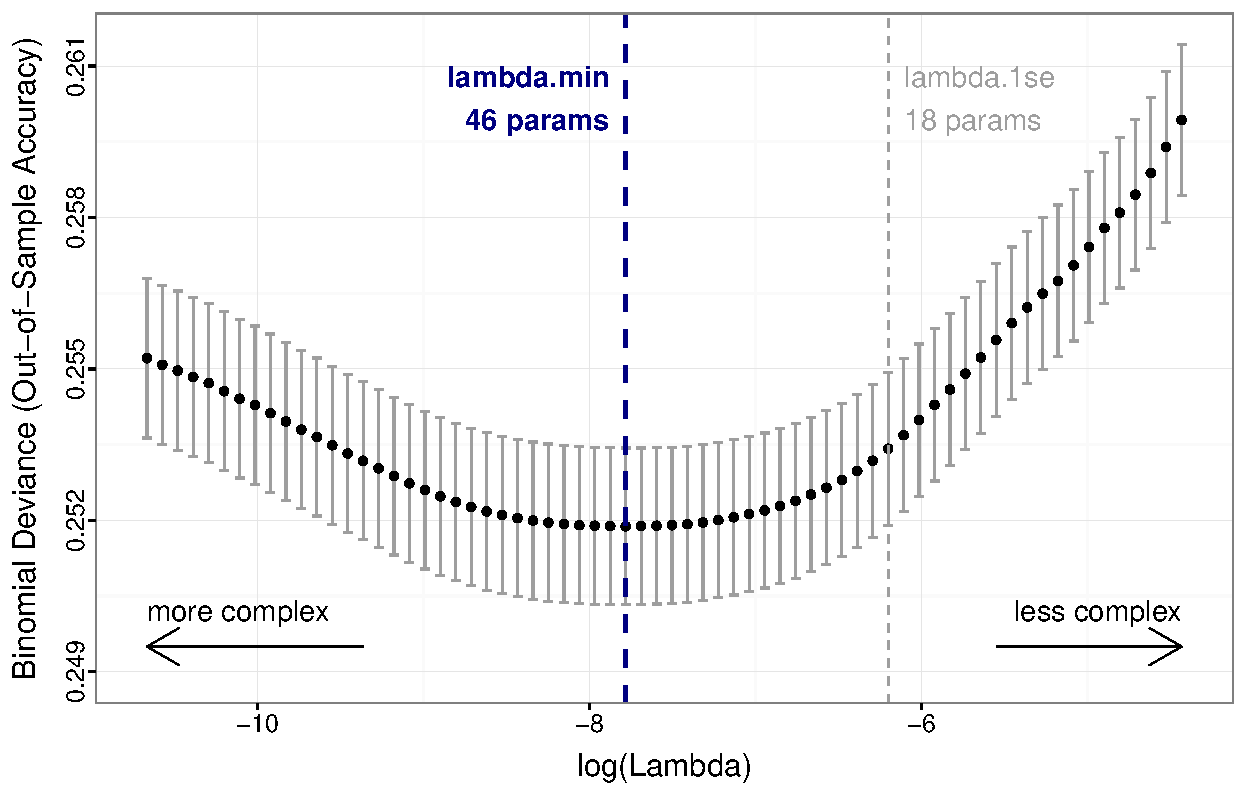
\includegraphics[width=\textwidth]{regpath1.pdf}
% \end{frame}

\begin{frame}
Trade-off between accuracy (\textit{\fg select variables via cross validation}) and simplicity/parsimony (\textit{\fg choose a small model})
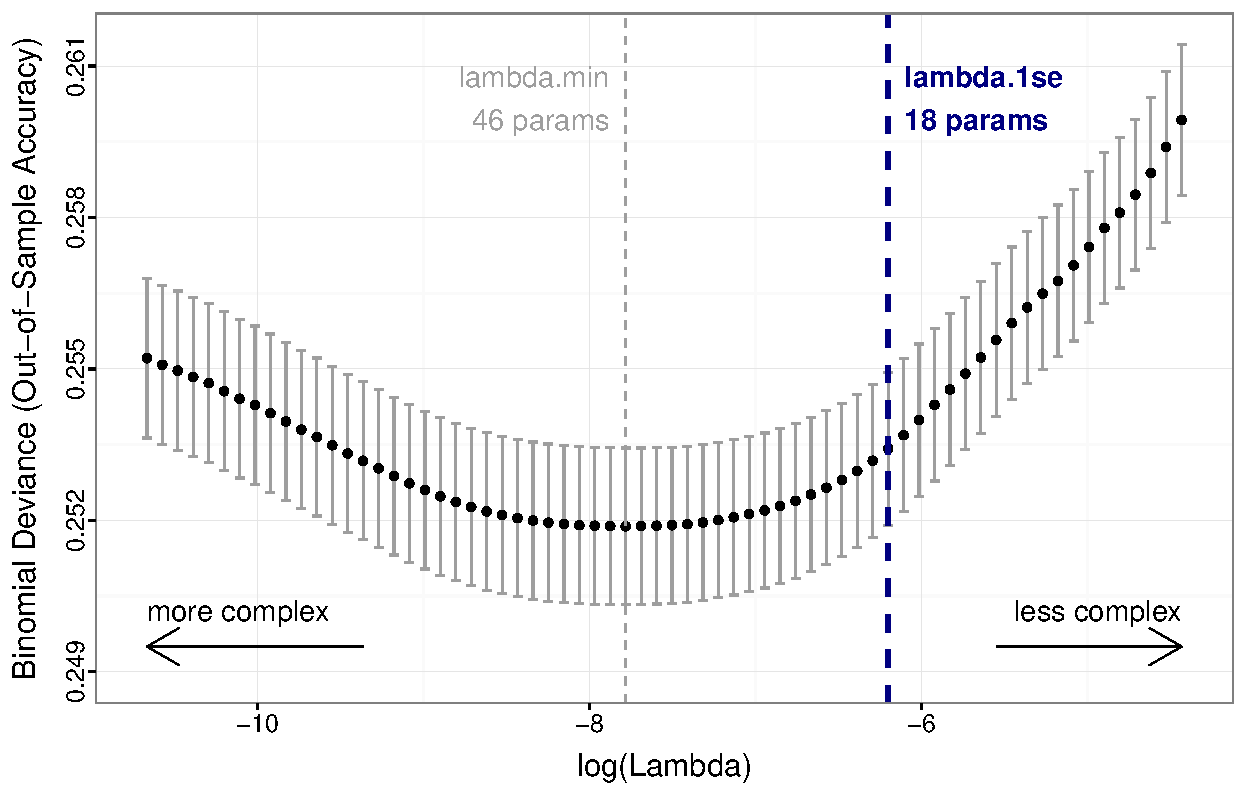
\includegraphics[width=\textwidth]{regpath2.pdf}
\end{frame}

\begin{frame}

\end{frame}

\end{document}
